% Generated from the public primitive catalog. Original Atlas drawing; Apache-2.0.
% Target: camellia-128; view: detail
\documentclass[border=9pt]{standalone}
% Original Atlas figure theme. Apache-2.0; see the repository LICENSE.
\usepackage[T1]{fontenc}
\usepackage{lmodern}
\usepackage{amsmath,amssymb}
\usepackage{tikz}
\usetikzlibrary{arrows.meta,positioning,calc,fit,backgrounds,decorations.pathreplacing,matrix}
\definecolor{atlasInk}{HTML}{172235}
\definecolor{atlasTeal}{HTML}{0D7B7D}
\definecolor{atlasMuted}{HTML}{637278}
\definecolor{atlasFill}{HTML}{EAF4F2}
\definecolor{atlasLine}{HTML}{B6C8C7}
\tikzset{
  every picture/.style={line width=.65pt,draw=atlasInk,>=Latex},
  every node/.style={text=atlasInk,font=\sffamily\small},
  box/.style={draw,rounded corners=1.5pt,minimum height=.9cm,minimum width=1.6cm,align=center,inner sep=6pt,fill=white},
  accent/.style={box,draw=atlasTeal,fill=atlasFill},
  wire/.style={->,line width=.7pt},
  keywire/.style={wire,draw=atlasTeal,dashed},
  xor/.style={draw,circle,fill=white,inner sep=0pt,minimum size=.38cm},
  add/.style={draw,rectangle,fill=white,inner sep=0pt,minimum size=.38cm},
  note/.style={font=\sffamily\scriptsize,text=atlasMuted,align=center},
  phase/.style={font=\sffamily\small\bfseries,text=atlasTeal},
  group/.style={draw=atlasLine,dashed,rounded corners=2pt,inner sep=8pt}
}
\newcommand{\rotl}{\mathbin{\lll}}
\newcommand{\rotr}{\mathbin{\ggg}}
\newcommand{\kx}{\operatorname{Keccak}\!\text{-}\!f[1600]}

\newcommand{\AtlasKeyBits}{128}
\newcommand{\AtlasKeyWords}{4}
\newcommand{\AtlasRounds}{18}
\newcommand{\AtlasPriorRounds}{17}
\newcommand{\AtlasRoundKeys}{19}
\newcommand{\AtlasDoubleRounds}{9}
\newcommand{\AtlasSixRoundGroups}{3}
\newcommand{\AtlasFLGroups}{2}
\newcommand{\AtlasRoundStart}{6}
\newcommand{\AtlasBlockBits}{128}
\newcommand{\AtlasOutputBits}{d}
\newcommand{\AtlasStateBits}{8w}
\newcommand{\AtlasNonceBits}{v}
\newcommand{\AtlasCounterBits}{q}
\newcommand{\AtlasStreamBlockBits}{b}
\newcommand{\AtlasRate}{r}
\newcommand{\AtlasCapacity}{c}
\newcommand{\AtlasSteps}{N}
\newcommand{\AtlasLastStep}{N-1}
\newcommand{\AtlasWordBits}{w}
\newcommand{\AtlasHashWords}{h}
\newcommand{\AtlasFeedForward}{\boxplus}
\newcommand{\AtlasByteOrder}{big-endian}
\newcommand{\AtlasDomain}{01}
\newif\ifAtlasXof
\AtlasXoffalse
\begin{document}
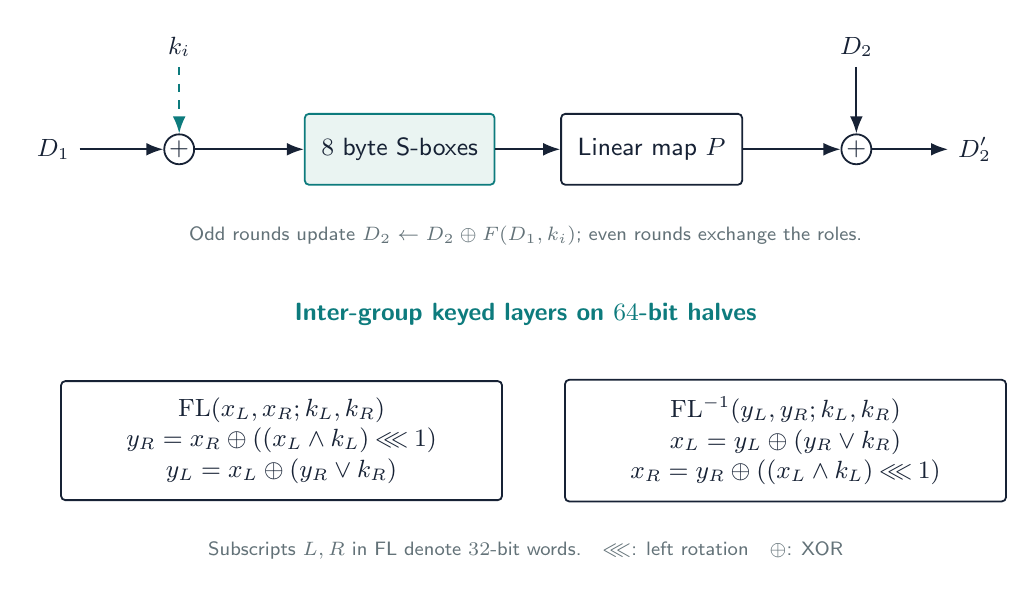
\begin{tikzpicture}
  \node (left) at (0,2) {$D_1$};
  \node[xor] (key) at (1.6,2) {$+$};
  \node[accent] (s) at (4.4,2) {$8$ byte S-boxes};
  \node[box] (p) at (7.6,2) {Linear map $P$};
  \node[xor] (xor) at (10.2,2) {$+$};
  \node (out) at (11.7,2) {$D'_2$};
  \draw[wire] (left) -- (key); \draw[wire] (key) -- (s); \draw[wire] (s) -- (p); \draw[wire] (p) -- (xor); \draw[wire] (xor) -- (out);
  \node (k) at (1.6,3.3) {$k_i$}; \draw[keywire] (k) -- (key);
  \node (right) at (10.2,3.3) {$D_2$}; \draw[wire] (right) -- (xor);
  \node[note] at (6,.9) {Odd rounds update $D_2\gets D_2\oplus F(D_1,k_i)$; even rounds exchange the roles.};
  \node[phase] at (6,-.1) {Inter-group keyed layers on $64$-bit halves};
  \node[box,minimum width=5.6cm] at (2.9,-1.7) {$\mathrm{FL}(x_L,x_R;k_L,k_R)$\\$y_R=x_R\oplus((x_L\land k_L)\rotl1)$\\$y_L=x_L\oplus(y_R\lor k_R)$};
  \node[box,minimum width=5.6cm] at (9.3,-1.7) {$\mathrm{FL}^{-1}(y_L,y_R;k_L,k_R)$\\$x_L=y_L\oplus(y_R\lor k_R)$\\$x_R=y_R\oplus((x_L\land k_L)\rotl1)$};
  \node[note] at (6,-3.1) {Subscripts $L,R$ in FL denote $32$-bit words.\quad $\rotl$: left rotation\quad $\oplus$: XOR};
\end{tikzpicture}

\end{document}
